\documentclass[english]{sareport}
% use the option peerreview for creating an anonymized version of your report
% E.g., \documentclass[english,peerreview]{sareport}

\usepackage[colorlinks, linkcolor=black, citecolor=black, urlcolor=black]{hyperref}
\usepackage{fontawesome}
\usepackage[normalem]{ulem}

\usepackage{graphicx}
\usepackage{rotating}
\usepackage{float}
\usepackage{enumitem}
\setlist{noitemsep} % \setlist{nosep}

% Set all authors, if your group counts 2, set third author empty \authorthree{}
% Set the groupname as well
\authorone{Monika Filipcikova (r0683254)}
\authortwo{Armin Halilovic(r0679689)}
\authorthree{}
\groupname{Filipcikova-Halilovic}
\academicyear{2016--2017}

\casename{Shared Internet Of Things Infrastructure Platform}
\phasenumber{2b}
\phasename{The Complete Architecture}

\begin{document}
\maketitle

\tableofcontents
% the following two command are necessary for obtaining the mini list of figures in the cs-view, decomposition view, deployment view and scenarios chapters
\dominilof
\fakelistoffigures

\chapter{Architectural Decisions}\label{ch:overview}
    % \chapter{Architectural Decisions}\label{ch:overview}

\section{Av1: Communication between SIoTIP gateway and Online Service}

    \todoinline{Use this section structure for each requirement}

    \subsection*{Key Decisions}

        The \texttt{OnlineServiceMonitor} monitors the Gateway's connectivity to the Online Service.
        The \texttt{OnlineServiceBrokerMonitor} monitors the communication component on Gateways.

        \begin{itemize}
        	\item decision 1
        	\item \ldots
        \end{itemize}
        \emph{Employed tactics and patterns:} heartbeats, ping/echo


    \subsection*{Rationale}
        \paragraph{Av1: New Gateway responsibilities}
            The SIoTIP gateway is able to autonomously detect failures of its individual internal communication components.\\
            The Online Service should acknowledge each message sent by the SIoTIP gateway so that the gateway can detect failures.\\
            If an internal SIoTIP gateway component fails, the gateway first tries to restart the affected component.
            If the failure persists, the SIoTIP gateway reboots itself entirely. Note that the SIoTIP gateway,
            due to the occurred failure, cannot contact a system administrator itself.\\
            If (an internal communication component of) the Online Service or the communication
            channel has failed, the SIoTIP gateway will temporarily store all incoming pluggable data
            and any issued application commands internally.\\
            If the Online Service becomes unreachable, application parts running locally on the SIoTIP
            gateway continue to operate normally.\\
            The SIoTIP gateway will start synchronising with the Online service within 1 minute after the
            communication channel becomes available.\\
        
            The \texttt{OnlineServiceBroker} isolates communication-related concerns between Gateways and the Online Service
            along with GatewayBroker on the Online Service.Forwards requests from one party to the other and transmits results and 
            possible exceptions.
            The SIoTIP gateway is able to autonomously detect failures of its individual internal communication components.
            The  \texttt{OnlineServiceBrokerMonitor} monitors the communication component on Gateways. 
            If the communication component fails, the monitor tries to restart it. If the failure persists, 
            the gateway reboots itself entirely.\\
            The \texttt{BrokerLogic} handles all functionality related to communication. In the \texttt{OnlineServiceBroker} 
            are \texttt{RequestStore} and \texttt{OnlineServiceMonitor}. 

            The \texttt{OnlineServiceMonitor} monitors the Gateway's connectivity to the Online Service. It checks acknowledgement of each
            message sent by the SIoTIP gateway. If (an internal communication component of) the Online Service or the communication
            channel has failed, all requests to the Online Service will be stopped and stored in the \texttt{RequestStore}. An explicit command for this is not necessary,
            because the requests in the \texttt{RequestStore} will not be deleted, since no acknowledgements are received
            anymore from the Online Service. It can store at least 3 days of pluggable data before old data has to be overwritten. 
            After the monitor detects that a connection to the Online Service is possible
            again, it makes the gateway start synchronising again. When the Online Service is unreachable, application 
            parts running locally on the SIoTIP gateway continue to operate normally.
            
            
        \paragraph{Av1: New Online Service responsibilities}
            The Online Service is able to autonomously detect failures of its individual internal communication components.\\
            The Online Service is able to detect that a SIoTIP gateway is not sending data anymore based on the expected synchronisation interval.\\
            The Online Service notifies the infrastructure manager and a SIoTIP system administrator when the outage of a SIoTIP gateway is detected.\\
            The failure of an internal SIoTIP Online Service component is detected within 30 seconds.\\
            The detection time for a failed SIoTIP gateway or channel depends on the transmission rate
            of the gateway. An outage is defined as 3 consecutive expected synchronisations that do not
            arrive within 1 minute of their expected arrival time.\\
            The infrastructure owner is notified within 5 minutes after the detection of an outage of their gateway.\\
            A SIoTIP system administrator should be notified within 1 minute after the detection
            of a simultaneous outage of more than 1\% of the registered gateways.\\

            GatewayBroker: Isolates communication-related concerns between the Online Service Gateways and along with OnlineServiceBroker on Gateways.
                       Forwards requests from one party to the other and transmits results and possible exceptions. \\
                       Sends acknowledgements for all messages sent by Gateways so that they can detect failures.
            GatewayBrokerMonitor: Monitor the communication component for communication with gateways on the Online Service.

            In GatewayBroker:
                BrokerLogic: Handles all functionality related to communication.
                GatewayMonitor: Monitors the connectivity status all gateways. Can detect that a gateway is not sending data anymore based on the expected synchronisation interval. If 3 consecutive expected synchronisations do not arrive within 1 minute of their expected arrival time,
                            this is detected as a gateway outage. When outages of gateways are detected, the infrastructure owners that own the gateways and a SIoTIP system administrator are notified.
                            When the connectivity status change of a Gateway is detected, this is saved in the DeviceDB.



    \subsection*{Considered Alternatives}
         Alternative for monitoring of gateways:
        Gateway updated come to GatewayMonitor
        We could make GatewayMonitor ping all the gateways
        However, this would increase traffic on the network

    \subsection*{Deployment Decisions}
        OnlineServiceBroker
        OnlineServiceBrokerMonitor

        GatewayBroker
        GatewayBrokerMonitor

        For both the Online Service and Gateways, the components used for communication
        (\texttt{OnlineServiceBroker}, \texttt{GatewayBroker}) are to be deployed on different nodes than
        their monitoring components (\texttt{OnlineServiceBrokerMonitor}, \texttt{GatewayBrokerMonitor}).
        Otherwise, if the node of a communication
        component fails, its monitoring component would also fail and thus
        nothing would be detected.

    \subsection*{Considered Deployment Alternatives}
        \ldots

\newpage
\section{Av2: Application failure}

    \subsection*{Key Decisions}

        \begin{itemize}
        	\item \texttt{ApplicationInstance}s are executed within \texttt{ApplicationContainer}s.
            \item \texttt{ApplicationContainerManager} creates/destroys/handles communication for \texttt{ApplicationContainer}s.
            \item \texttt{ApplicationContainerMonitor} monitors \texttt{ApplicationContainer}s and \texttt{ApplicationInstance}s.
            \item \texttt{ApplicationExecutionSubsystemMonitor} monitors the application execution subsystem.
        \end{itemize}
        \emph{Employed tactics and patterns:} container

    \subsection*{Rationale}
        To handle Av2, we developed the whole application execution subsystem in a decomposition
        with Av2 and important application instance related use cases. The application execution subsystem
        is composed of the following components:
        \begin{itemize}
            \item \texttt{ApplicationContainer}
            \item \texttt{ApplicationContainerMonitor}
            \item \texttt{ApplicationContainerManager}
            \item \texttt{ApplicationExecutionSubsystemMonitor}
            \item \texttt{DeviceDataConverter}
            \item \texttt{DeviceCommandConstructor}
        \end{itemize}

        Av2 states "The system is able to autonomously detect failures of its individual
        application execution components, failing applications, and failing application containers.".\\
        These responsibilities are handled by the \texttt{ApplicationContainer}, \texttt{ApplicationContainerMonitor}, and \texttt{ApplicationExecutionSubsystemMonitor}.
        The \texttt{ApplicationContainer} provides a sandbox environment for an \texttt{ApplicationInstance} to run in and has the ability
        to monitor the instance. When an application instance fails, the container notifies the \texttt{ApplicationContainerMonitor} of this.\\
        Next to this, the \texttt{ApplicationContainerMonitor} pings \texttt{ApplicationContainer}s regularly to check whether or not the container
        has failed. If a failure of an application instance/container is detected, the \texttt{ApplicationContainerMonitor} sends a command to the
        \texttt{ApplicationContainerManager} to restart the instance/container or to create a new one in case the first two restarts did not work.
        If the application instance then keeps failing, it is suspended and the application provider and affected customer organisation are notified.
        When an application fails, a message of this is sent to the other parts of the application, so that they can possible run in a degraded mode. \\
        The \texttt{ApplicationContainerMonitor} also keeps track of how many times an \texttt{ApplicationInstance} has failed, so that when the container
        fails, there also is data about the instance.\\
        Lastly, the \texttt{ApplicationExecutionSubsystemMonitor} monitors other parts of the application execution subsystem, and restarts them
        in case failure is detected. \\

        Because of how different \texttt{ApplicationInstance}s run each in their own \texttt{ApplicationContainer}, no other applications or availability
        of other functionality of the system is affected.

    \subsection*{Deployment Decisions}
        For Av2, is important that \texttt{ApplicationInstance}s are deployed on different node from the \texttt{ApplicationContainerMonitor} that is responsible for
        monitoring. If the node the \texttt{ApplicationInstance} fails, then the \texttt{ApplicationContainerMonitor} won't also automatically fail with the \texttt{ApplicationInstance}
        and interested parties can be informed. \\
        In order to make sure that no applications or functionality of the system is affected when an application instance/container fails, each \texttt{ApplicationContainer}
        runs on its own node. The \texttt{ApplicationContainerManager} keeps track of all \texttt{ApplicationContainer}s.

\newpage
\section{Av3: Pluggable device or mote failure}

    \todoinline{Use this section structure for each requirement}

    \subsection*{Key Decisions}

    \todoinline{
    	Briefly list your key architectural decisions.
    	Pay attention to the solutions that you employed (in your own terms or using tactics and/or patterns).
    }

    \begin{itemize}
    	\item \texttt{DeviceManager} monitors connected/operational devices on a gateway.
    	\item \texttt{DeviceManager} stores the requirements for pluggable devices set by applications
    \end{itemize}
    \emph{Employed tactics and patterns:} heartbeat, ping/echo

    \subsection*{Rationale}
        \paragraph{Failure detection}
            Gateway need to be able to autonomously detect failure of one of its
            connected motes and pluggable devices. This is achieved by making motes
            send heartbeats to their connected gateways. The gateways can
            then monitor their connected devices. The heartbeats contain a list
            of devices that are connected/operational at the moment the mote sends
            the heartbeat. Each gateway makes use of a \texttt{DeviceManager}
            component to monitor the devices. This component uses timers to keep track
            of how long it has been since a device has sent a heartbeat or occured in
            a list of connected devices. Once a timer expires, this is treated as
            a failure. \\

            A mote has failed when 3 consecutive heartbeats do not arrive within 1
            second of their expected arrival time. \\
            A pluggable device has failed when it does not occur in a heartbeat of the
            mote in which it is expected to be in. This is is detected within 2
            seconds after the arrival of the heartbeat.

        \paragraph{Automatic application deactivation and redundancy settings}
            Applications should be automatically suspended when they can no longer
            operate due to failure of a pluggable device or mote and reactivated
            once the failure is resolved. Application providers can design their
            applications such that they explicitly require redundancy in
            the available pluggable devices. \\
            This problem is tackled by the \texttt{DeviceManager}. It
            stores the requirements for pluggable devices set by applications for all
            applications that use the gateway that the \texttt{DeviceManager}
            runs on. When it detects that an application can no longer operate
            due to failures, it will send a command to the \texttt{ApplicationManager}
            (via the \texttt{GatewayFacade})
            to suspend that application. When the required devices are operational
            again, the \texttt{DeviceManager} detects this and sends a
            command to reactivate the application. \\

            Applications are suspended within 1 minute after detecting
            the failure of an essential pluggable device. \\
            Application are reactivated within 1 minute after the failure is resolved.

        \paragraph{Notifications}
            The infrastructure owner should be notified of any persistent
            pluggable device or mote failures. Customer organisations should be
            notified if one or more of their applications is suspended or
            reactivated. Applications using a failed pluggable device or any device
            on a failed mote should be notified. \\
            The \texttt{NotificationHandler} was put in place to deal with
            notifications. Other components can use it to generate notifications for
            certain users in the system. The \texttt{NotificationHandler} will then
            insert information relevant to the notification in the database (message,
            status, date and time, source, ...), and use an external delivery
            service to deliver the notification to users. The used delivery medium
            is based on the user's preferences. The \texttt{DeviceManager} sends request
            to the external delivery service to notifies the
            infrastructure owner, once mote or pluggable device failure occurs.
            Since they are stored in the database, users can always view
            their notifications via their dashboard. However, this funcionality is not
            expanded on in this decomposition yet. \\

            Infrastructure owners are notified within 1 minute after detecting a mote outage lasting at
            least 10 seconds. \\
            Infrastructure owners are notified within 1 minute after the detection of the unavailability of
            a pluggable device for 30 seconds. \\
            Applications are notified of the failure of relevant pluggable devices within 10 seconds.


    \subsection*{Considered Alternatives}
        \paragraph{Alternative for failure detection}
            An alternative would have been to move the \texttt{DeviceManager}
            component from gateways to the Online Service. This solution would make the
            gateways do less work, but would be very unscalable. The reason is
            that as the customer base (and thus the amount of devices) increases,
            the Online Service would need to keep track of huge amounts of devices.
            This would also flood the network to the Online Service with heartbeats.

        \paragraph{Alternative for Failure detection}
            Another alternative for failure detection could have been the use of
            a Ping/Echo mechanism instead of Heartbeats. Pings could then be used
            to check if a device is currently operational. However, as a device could
            not be operational for a moment because of e.g. interference, timers
            would still be necessary to keep track of operational devices. We opted
            to use heartbeats, as this would reduce the amount of data sent over
            the network used by the motes, and as motes would have to do slightly
            more work to process each Ping request in order to generate a reply.

        \paragraph{Av3: Notifications}
            Reliable and quick delivery of notifications is crucial to the
            system in order to solve problems should things go wrong. Currently,
            the solution is to use a third party service for delivery of
            notifications. In the case that no external services are found
            satisfactory, or if this dependency on an external service is
            unwanted, it is possible to build an internal solution for this.
            For example, a \texttt{NotificationSender} component could make use
            of the \texttt{Factory pattern} for different message channels for
            different delivery methods (each with their own sendNotification method).
            This solution allows us to easily add new message channels in the
            future with little effort. The disadvantage of this is that an
            internal solution takes a lot more time to implement.


    \subsection*{Deployment Decisions}
        For Av3 is important that the \texttt{DeviceManager} is deployed on another node as the
        \texttt{Mote} and the \texttt{PluggableDevice}. The \texttt{DeviceManager}
        checks the \texttt{Mote} and the \texttt{PluggableDevice} availability and in case of failure, the \texttt{DeviceManager}
        can notify the infrastructure owner of any persistent pluggable device or mote failures.\\

\newpage
\section{M1: Integrate new sensor or actuator manufacturer}

    \subsection*{Key Decisions}

    \begin{itemize}
    	\item Modifiability is maintained by splitting up functionality that would need to be updated
              when new pluggable devices are introduced to the system into different components.
        \item In interfaces, pluggable devices are only referred to by their unique PluggableDeviceID,
              types and other device info is left out of parameter lists.
              
    \end{itemize}
    \emph{Employed tactics and patterns:} None

    \subsection*{Rationale}
        \paragraph{M1: Data conversion}
            With new types of devices, the pluggable data processing subsystem
            should be extended with relevant data conversions,
            e.g. converting temperature in degrees Fahrenheit to degrees Celsius. \\
            The \texttt{DeviceDataConverter} is put in place to handle the
            task of converting pluggable device data to data of a different type in the system.
            This component can easily be modified for new types of data simply by
            adding a new conversion method for the new.

        \paragraph{M1: Usage of new data by applications}
            The available applications in the system can be updated to use any
            new pluggable devices. \\
            This is made possible by the RequestData
            interface provided by \texttt{DeviceDataScheduler}.
            Data of the new type of device can be requested in the same way
            as for older devices: by using the device's unique id.
            The application manager can get pluggable device data from the
            \texttt{PluggableDeviceDataDB} and return this data to applications in
            the DeviceData datatype. This datatype can easily be
            updated for new types of pluggable devices.

        \paragraph{P2: Scheduling}
            The pluggable data processing subsystem needs to be able to run in normal
            or overload mode, depending on whether or not the system can process
            requests within the deadlines given in the quality requirement. Also,
            a mechanism should be in place to avoid starvation of any type of request. \\
            The \texttt{DeviceDataScheduler} is used to deal with this problem.
            It is responsible for scheduling requests that wish to interact with
            the \texttt{PluggableDeviceDataDB}. In normal mode, the system processes
            incoming requests in a FIFO order. In overload mode, the requests are
            given a priority based on what the request is for and what the source
            of the request is. The requests are then not simply processed in an
            order based on their priorities, but an aging technique is to be used
            such that starvation will be avoided. Thus, in overload mode,
            requests are processed in an order based on a combination of the
            priorities of the requests and the age of the requests.

        \paragraph{P2: Pluggable data separation}
            The processing of (large amounts of) requests concerning pluggable
            data has no impact on requests concerning other data, e.g. available applications. \\
            In order to statisfy this constraint, all data directly related to
            pluggable data has been separated into the \texttt{PluggableDeviceDataDB}.
            All requests concerning pluggable data will be handled by this new
            component. \texttt{PluggableDeviceDataDB} will run on a node different
            from the node that the \texttt{Datbase} component runs on. This way
            requests concerning pluggable will have no impact on
            requests concerning other data.

        \paragraph{M1: Handling new types of pluggable devices}
            The new types of sensor or actuator data should be transmitted,
            processed and stored, and should be made available to applications.
            The infrastructure managers must be able to initialize the new type
            of pluggable device, configure access rights for these devices, and
            view detailed information about the new type of pluggable device. \\
            The components created thus far have been created with high cohesion in
            mind so that updating them for new devices would be relatively straightforward.
            In order for this constraint to be satisfied, changes have to be made to
            the following elements:
            \begin{itemize}
                \item \emph{PluggableDevice}: This component needs to be updated
                      so that the new type of device can be initialised and configured,
                      and thus so that the device's data can be sent to the system.
                \item \emph{DeviceData}: Depending on how this data type
                      is implemented, it might need an update in order for it
                      to represent possible new data types (for example
                      Temperature Filipcikova) and for the new data types to be
                      serialized.
                \item \emph{PluggableDeviceDataDB}: The database needs to be updated
                      so that information can be retrieved about the new types
                      of sensors and the new types of data. Data related to the
                      displaying of sensor data will also need to be updated.
                \item \emph{PluggableDeviceConverter}: see above.
            \end{itemize}

    \subsection*{Considered Alternatives}
        \paragraph{Alternative(s) for choice 1} Explain what alternative(s) you
        considered for this design choice and why they where not selected.

    \subsection*{Deployment Decisions}
        \ldots

    \subsection*{Considered Deployment Alternatives}
        \ldots

\newpage
\section{P1: Large number of users}
    \todoinline{Use this section structure for each requirement}
    \subsection*{Key Decisions}
    \todoinline{
    	Briefly list your key architectural decisions.
    	Pay attention to the solutions that you employed (in your own terms or using tactics and/or patterns).}
    \begin{itemize}
    	\item decision 1
    	\item \ldots
    \end{itemize}
    \emph{Employed tactics and patterns:} \ldots

    \subsection*{Rationale}
    \todoinline{Describe the design choices related to \emph{ReqX} together with the rationale
    	of why these choices where made.}

    \subsection*{Considered Alternatives}
    \paragraph{Alternative(s) for choice 1} Explain what alternative(s) you
    considered for this design choice and why they where not selected.

    \subsection*{Deployment Decisions}
    \ldots

    \subsection*{Considered Deployment Alternatives}
    \ldots


\newpage
\section{P2: Requests to the pluggable data database}

    \subsection*{Key Decisions}

        \begin{itemize}
            \item \texttt{PluggableDeviceDataDB} separates the requests concerning pluggable data
                  so that those requests have no impact on requests concerning other data.
        	\item \texttt{DeviceDataScheduler} handles all requests for the \texttt{PluggableDeviceDataDB},
                  recognizes when the data processing subsystem needs to run in normal or overload mode,
                  and prevents starvation of requests.
        \end{itemize}
        \emph{Employed tactics and patterns:} \ldots

    \subsection*{Rationale}
        \paragraph{P2: Scheduling}
            The pluggable data processing subsystem needs to be able to run in normal
            or overload mode, depending on whether or not the system can process
            requests within the deadlines given in the quality requirement. Also,
            a mechanism should be in place to avoid starvation of any type of request. \\
            The \texttt{PluggableDeviceDataScheduler} is used to deal with this problem.
            It is responsible for scheduling requests that wish to interact with
            the \texttt{PluggableDeviceDB}. In normal mode, the system processes
            incoming requests in a FIFO order. In overload mode, the requests are
            given a priority based on what the request is for and what the source
            of the request is. The requests are then not simply processed in an
            order based on their priorities, but an aging technique is to be used
            such that starvation will be avoided. Thus, in overload mode,
            requests are processed in an order based on a combination of the
            priorities of the requests and the age of the requests.

        \paragraph{P2: Pluggable data separation}
            The processing of (large amounts of) requests concerning pluggable
            data has no impact on requests concerning other data, e.g. available applications. \\
            In order to statisfy this constraint, all data directly related to
            pluggable data has been separated into the \texttt{PluggableDeviceDB}.
            All requests concerning pluggable data will be handled by this new
            component. \texttt{PluggableDeviceDB} will run on a node different
            from the node that the \texttt{Datbase} component runs on. This way
            requests concerning pluggable will have no impact on
            requests concerning other data.

    \subsection*{Considered Alternatives}
        \paragraph{Alternative(s) for choice 1} Explain what alternative(s) you
        considered for this design choice and why they where not selected.

    \subsection*{Deployment Decisions}
        \ldots

    \subsection*{Considered Deployment Alternatives}
        \ldots

\newpage
\section{U2: Easy installation}

    \todoinline{Use this section structure for each requirement}

    \subsection*{Key Decisions}

        \todoinline{
        	Briefly list your key architectural decisions.
        	Pay attention to the solutions that you employed (in your own terms or using tactics and/or patterns).
        }

        \begin{itemize}
        	\item decision 1
        	\item \ldots
        \end{itemize}
        \emph{Employed tactics and patterns:} \ldots

    \subsection*{Rationale}
        \todoinline{
            Describe the design choices related to \emph{ReqX} together with the rationale
        	of why these choices where made.
        }

    \subsection*{Considered Alternatives}
        \paragraph{Alternative(s) for choice 1} Explain what alternative(s) you
        considered for this design choice and why they where not selected.

    \subsection*{Deployment Decisions}
        \ldots

    \subsection*{Considered Deployment Alternatives}
        \ldots


\section{Other decisions}

    \subsection{Authentication}
        \subsubsection*{KeyDecisions}
            A database is used to store login sessions.

        \subsubsection*{Rationale}
            Authentication is done by verifying user credentials when a user wants to log in. Then a unique session
            is created and the sessionID of this session is returned to the client used by the user. In all subsequent requests,
            the user's client adds this sessionID with the request. If the sessionID exists in the database, then this means
            that the user is still logged in and the request can be handled. Every time the sessionID is checked in the database,
            a timestamp is reset. After a certain time without any requests for this sessionID, the session is deleted from the system. \\

            The \texttt{SessionDB} is used to store all sessions.

        \subsubsection*{Considered Alternatives}
            \paragraph{Files for sessions}
                The sessions could be stored as files on the UserFacade that handlers requests for a user. The facade could then check
                whether or not a certain file exists to check if a user is logged in. However, this would make the facades stateful and
                would add extra overhead in keeping the session files on different nodes consistent with each other in case that the
                user is redirected to another node for load balancing. Keeping different nodes for facades consistent is much easier
                if they are all stateless.

        \subsubsection*{Deployment Decisions}
            The \texttt{SessionDB} is to be deployed on a separate node in order to avoid puttting extra strain on the other databases.
            We expect the SessionDB to receive many more requests than e.g. the \texttt{OtherDataDB}, since users need to send a sessionID
            with every request so that it can be checked whether or not the user is (still) logged in.

    \subsection{Notifications}
        \subsubsection*{KeyDecisions}
            The NotificationHandler stores and sends notifications.

        \subsubsection*{Rationale}
            The \texttt{NotificationHandler} was put in place to deal with
            notifications. Other components can use it to generate notifications for
            certain users in the system. The \texttt{NotificationHandler} will then
            insert information relevant to the notification in the database (message,
            status, date and time, source, ...), and use an external delivery
            service to deliver the notification to users. The used delivery medium
            is based on the user's preferences. The \texttt{DeviceManager} sends request
            to the external delivery service to notifies the
            infrastructure owner, once mote or pluggable device failure occurs.
            Since they are stored in the database, users can always view
            their notifications via their dashboard. \\

        \subsubsection*{Considered Alternatives}
            \paragraph{Custom delivery solution}
                Reliable and quick delivery of notifications is crucial to the
                system in order to solve problems should things go wrong. Currently,
                the solution is to use a third party service for delivery of
                notifications. In the case that no external services are found
                satisfactory, or if this dependency on an external service is
                unwanted, it is possible to build an internal solution for this.
                For example, a \texttt{NotificationSender} component could make use
                of the \texttt{Factory pattern} for different message channels for
                different delivery methods (each with their own sendNotification method).
                This solution allows us to easily add new message channels in the
                future with little effort. The disadvantage of this is that an
                internal solution takes a lot more time to implement.

    \subsection{Application execution subsystem}
        The application execution subsystem is composed of the following components:
        \begin{itemize}
            \item \texttt{ApplicationContainer}
            \item \texttt{ApplicationContainerMonitor}
            \item \texttt{ApplicationContainerManager}
            \item \texttt{ApplicationExecutionSubsystemMonitor}
            \item \texttt{DeviceDataConverter}
            \item \texttt{DeviceCommandConstructor}
        \end{itemize}

        \subsubsection*{Rationale}
            We have designed the application execution subsystem to use the same components on the Online Service and on Gateways,
            because we wanted reuse a lot of functionality in order to make everyones' lives a little easier. This seemed possible to us
            as it seemed to us that in the requirements there was not much different between the application instances running on Gateways
            and on the Online Service. \\
            The biggest difference is that because Gateways are weaker machines than the ones on the Online Service, the applications
            running on the gateways should be of smaller scales. This is perfectly possible by changing some configurations in the
            \texttt{ApplicationContainer}s so that they have stricter limits on the resources used of the node they are running on.
            If an application were to be too large or resource intensive, the \texttt{ApplicationContainerManager}'s 'testApplication' method
            could then generate error messages for the Gateway version of the application.\\
            Furthermore, to make this work smoothly, some interfaces used by the application execution subsystem would need to be
            re-routed to use (the same methods on) different interfaces of different components. For example, the \texttt{DeviceCommandConstructor}
            on the gateway should use the \texttt{DeviceManager} to fetch the correct formatting syntax of a pluggable device, instead of the \texttt{DeviceDB}.
            These things could also be done by using some specific configurations when deploying the components.

\section{Discussion}
    Overall, the architectural decisions lack alternative solutions and alternative deployments decisions.
    More research should be done about different ways to handle the
    non-functional requirements, in order to better judge and compare our solutions.\\

    In retrospect, we should have handled the DeviceDataConverter (and all components which rely on specific pluggable device information) differently.
    If we let data conversion methods be stored on the \texttt{DeviceDB}, we could let the DeviceDataConverter fetch those methods when necessary and maybe
    keep them in some kind of local cache. That way, the new methods can just be added in the database and the component would not need to be re-deployed.
    This is already done with pluggable device information on the \texttt{DeviceManager}; when it detects a new device, it loads information about the device
    and keeps it on the gateway while the device is connected to it.\\

    We should have decomposed the \texttt{DeviceManager} some more to show how device connectivity is being tracked with a \texttt{DeviceMonitor} and how
    applications' device usage/requirements data is stored in a \texttt{ApplicationDataStore}.\\

    Too much communication happens between Gateways and the Online Service, we should have let fewer requests happen between Gateways and the Online Service,
    and do more of the work on a \texttt{GatewayFacade} on the Online Service by doing different method calls from the \texttt{GatewayFacade} instead of \texttt{Gateway}s.

    In the rationale of P1, it is noticeable that the quality attribute has not been completely handled. \\

    In our design, we have not worked with states of application instances. Thus, if an application were to crash at some point, or if it would need to be shut down temporarily, etc.
    it would not be possible to save the state of an application and restore it at a later point. Maybe a simple solution for this would be to force application providers to
    implement a certain method so that the state of an application could be retrieved and stored. \\

    The \texttt{NotificationHandler} should have different notify methods for different situations, so that more details can be saved such as the cause of the notification.

    \clearpage

\chapter{Client-server view (UML Component diagram)}\label{ch:client-server}
    \minilof
    % \chapter{Client-server view (UML Component diagram)}\label{ch:client-server}

% Delete the command below to remove the hints and instructions
\showcsnotes{}

\section{Context diagram}
    The context diagram of the client-server view is displayed in figure \ref{fig:cc-context}. \\

    The external components are as follows.
    \begin{itemize}
        \item NotificationDeliveryService: blabla
        \item InfrastructureOwnerClient: blabla
        \item CustomerOrganisationClient: blabla
    \end{itemize}

    \todoinline{
    The context diagram of the client-server view:
    Discuss which components communicate with external components and what these external components represent.
    }


    \begin{landscape}
        \centering
        \vspace*{\fill}

        \begin{figure}[!htp]
            \centering
            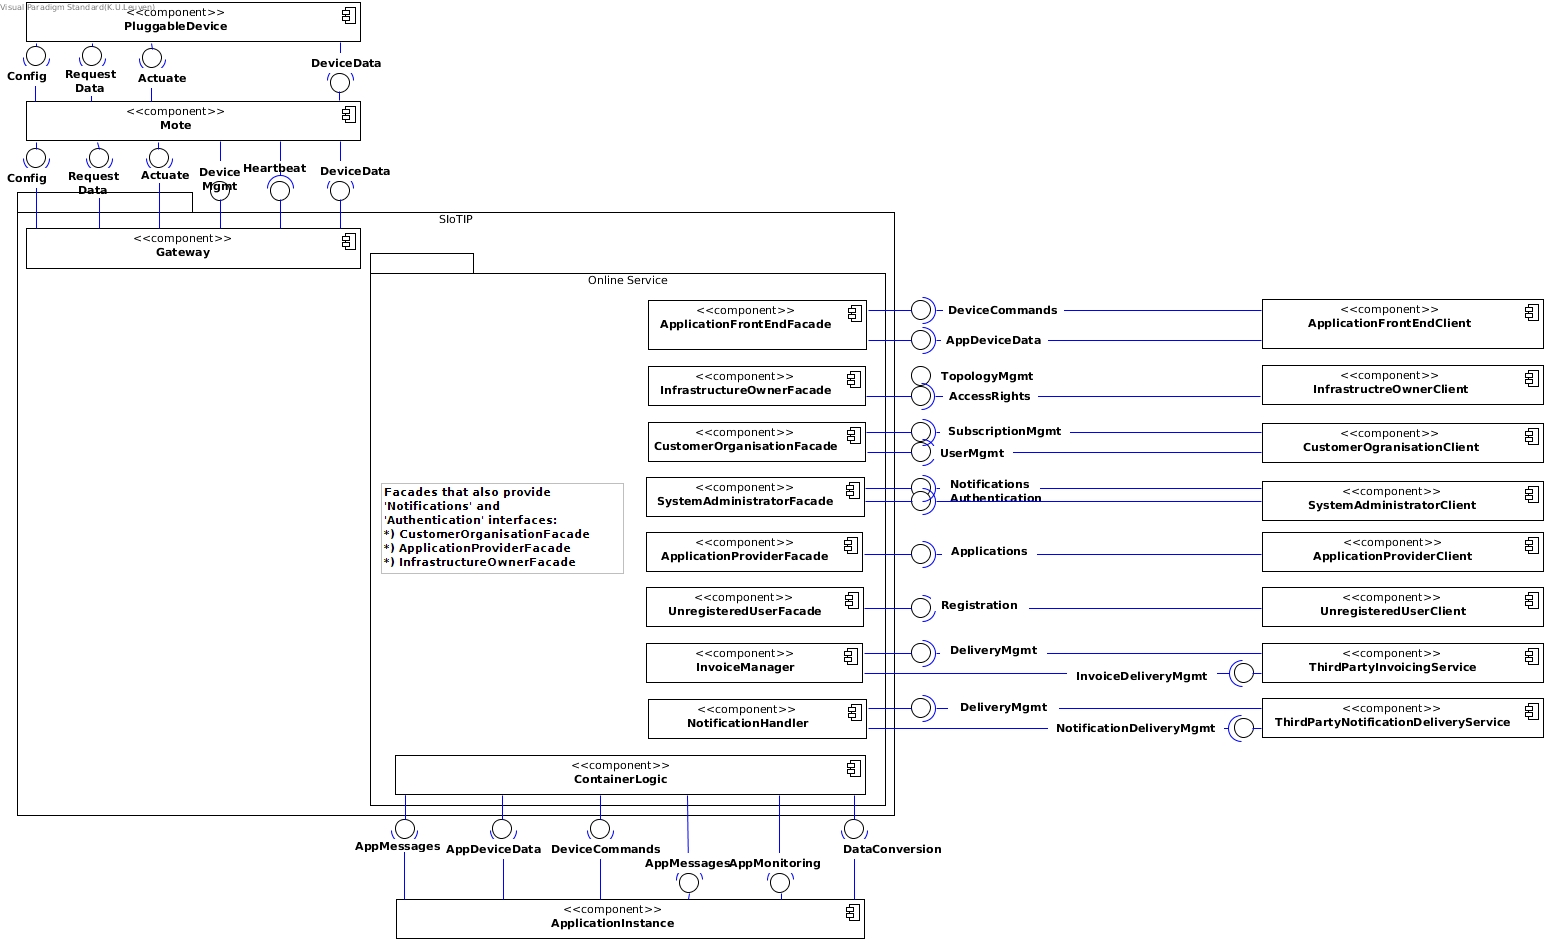
\includegraphics[width=\linewidth]{images/component-CONTEXT}
            \caption{Context diagram for the client-server view.}\label{fig:cc-context}
        \end{figure}

        \vfill
    \end{landscape}

\section{Primary diagram}
    The primary diagram of the client-server view is displayed in figure \ref{fig:cc-primary}. \\

    \todoinline{The primary diagram and accompanying explanation.}

    \begin{landscape}
        \centering
        \vspace*{\fill}

        \begin{figure}[!htp]
            \centering
            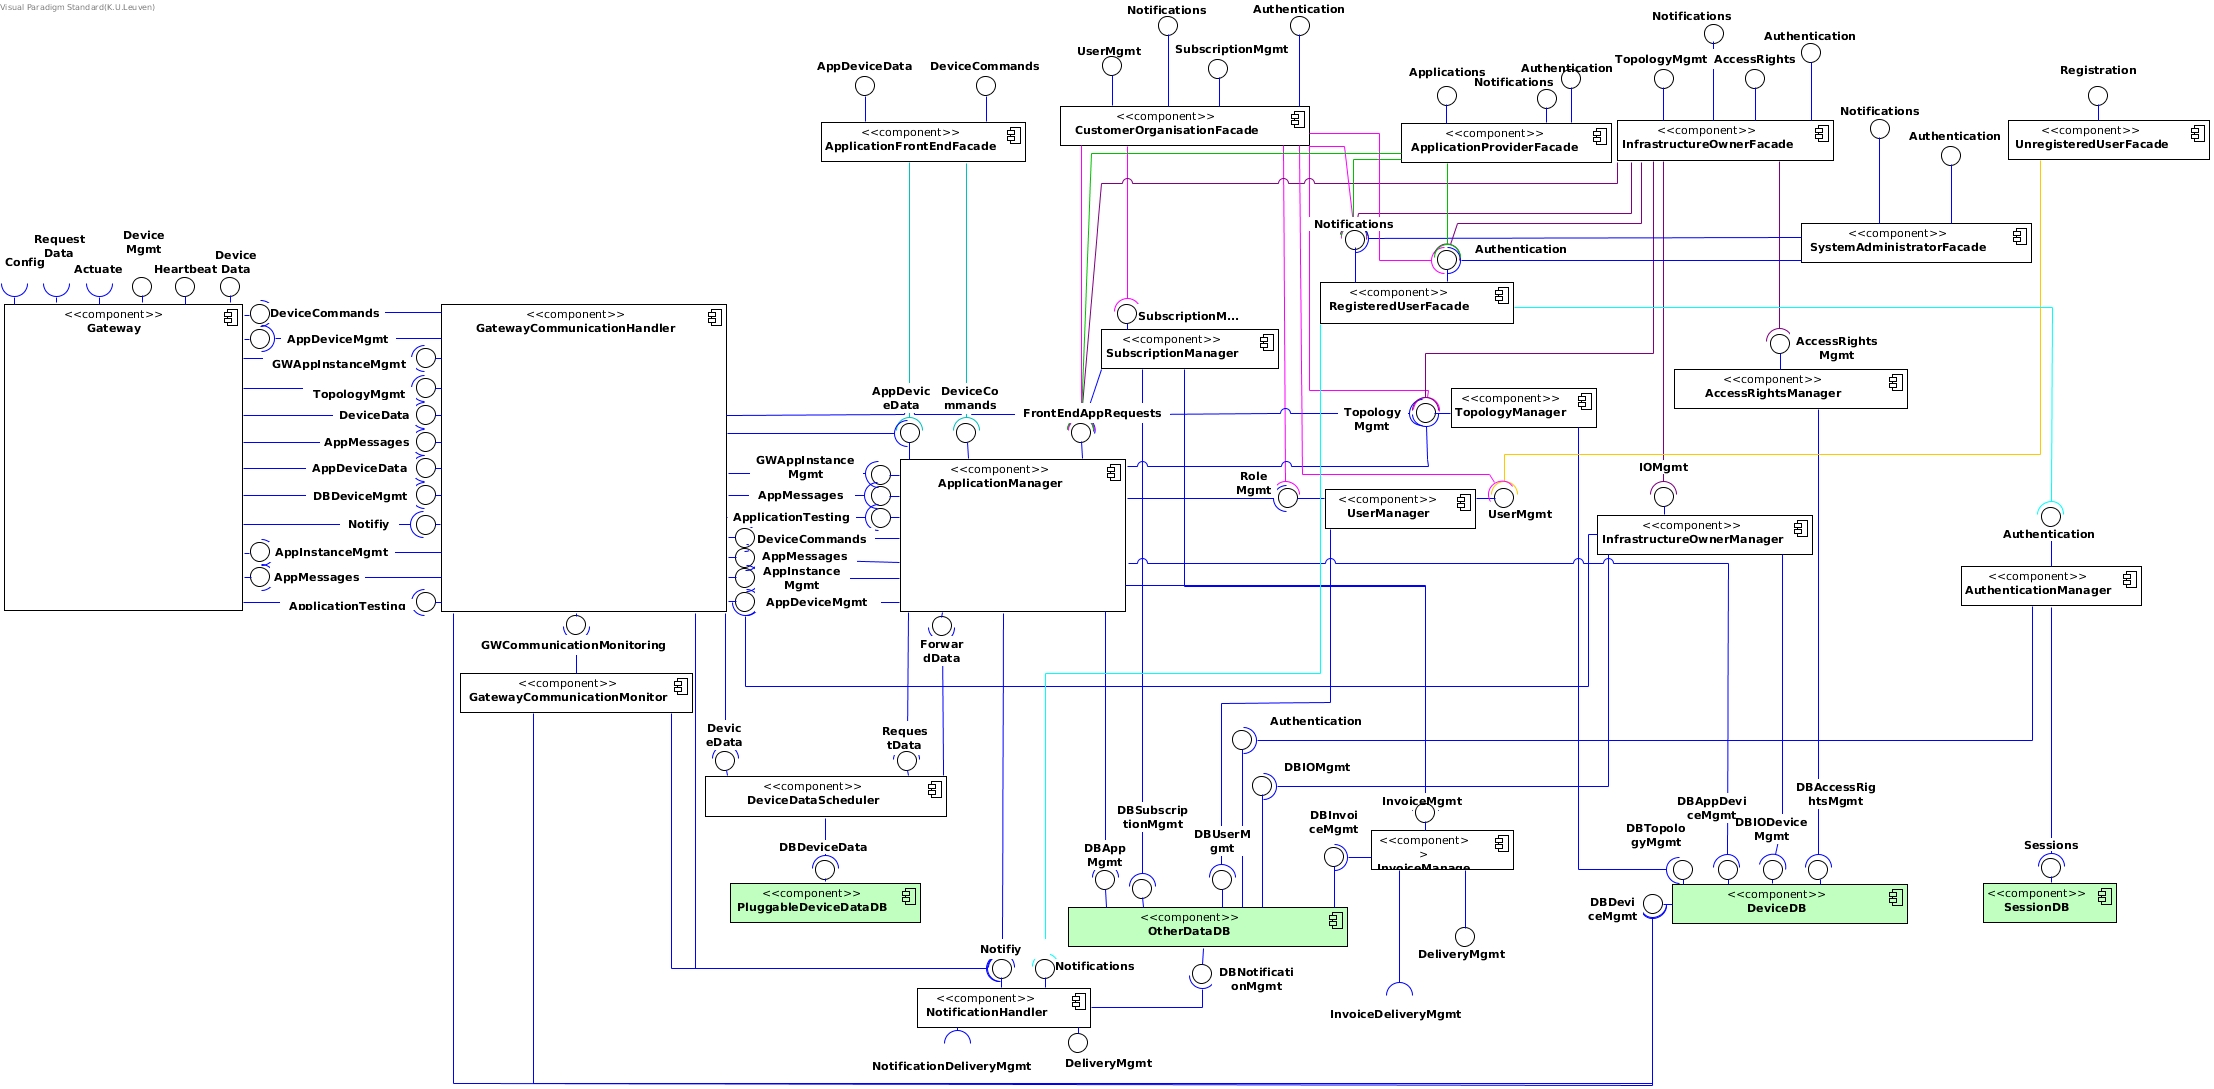
\includegraphics[width=\linewidth]{images/component-PRIMARY}
            \caption{Primary diagram of the client-server view.}\label{fig:cc-primary}
        \end{figure}

        \vfill
    \end{landscape}

    \clearpage

\chapter{Decomposition view (UML Component diagram)}\label{ch:decomposition}
    \minilof
    %\chapter{Decomposition view (UML Component diagram)}\label{ch:decomposition}

% Delete the command below to remove the hints and instructions
\showdecompnotes{}

\begin{figure}[!htp]
	\centering
	%\includegraphics[width=\textwidth]{}
	\missingfigure[figwidth=0.8\textwidth]{Diagram showing decomposition of ComponentX}
	\caption{Decomposition of \texttt{ComponentX}}\label{fig:decomp-componentx}
\end{figure}

\begin{figure}[!htp]
	\centering
	%\includegraphics[width=\textwidth]{}
	\missingfigure[figwidth=0.8\textwidth]{Diagram showing decomposition of ComponentX}
	\caption[Decomposition of \texttt{ComponentY}]{Decomposition of \texttt{ComponentY}.\\
	This caption contains a longer explanation over multiple lines. This additional explanation is not shown in the list of figures.}\label{fig:decomp-componenty}
\end{figure}

    \clearpage
    % \stoplist[decomp]{lof}

\chapter{Deployment view (UML Deployment diagram)}\label{ch:deployment}
    \minilof
    % \chapter{Deployment view (UML Deployment diagram)}\label{ch:deployment}


\begin{landscape}
    \section{Context diagram}
    The context diagram for the deployment view is displayed in figure \ref{fig:depl_context}. \\

    \centering
    \vspace*{\fill}

        \begin{figure}[!htp]
        	\centering
            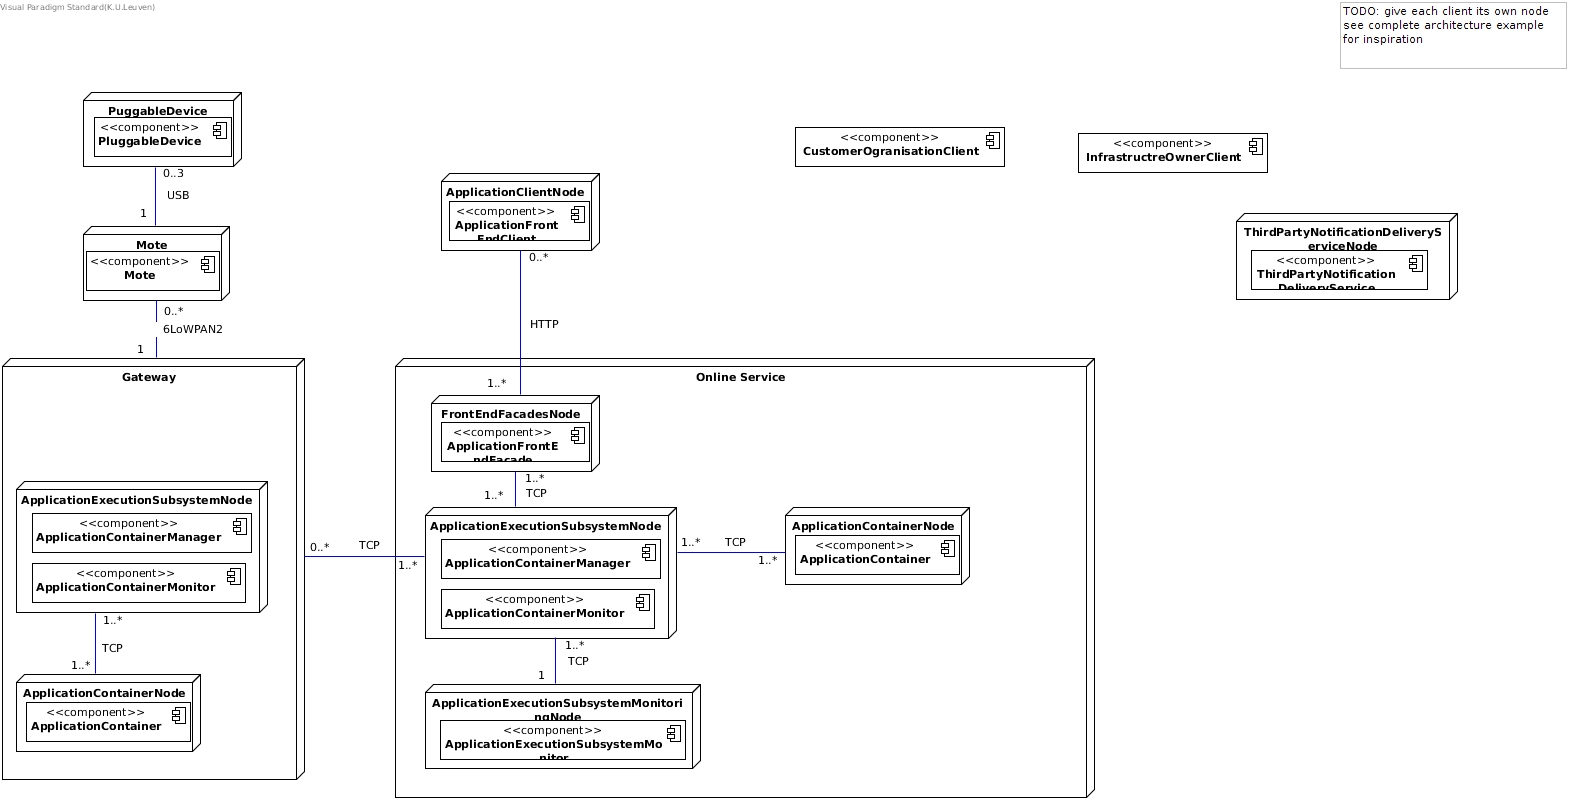
\includegraphics[width=\textwidth]{images/deployment-context}
            \caption{Context diagram for the deployment view.}\label{fig:depl_context}
        \end{figure}

    \vfill
\end{landscape}


\begin{landscape}
    \section{Primary diagram}
    The primary diagram for the deployment view is displayed in figure \ref{fig:depl_primary}.

    \centering
    \vspace*{\fill}

        \begin{figure}[!htp]
        	\centering
            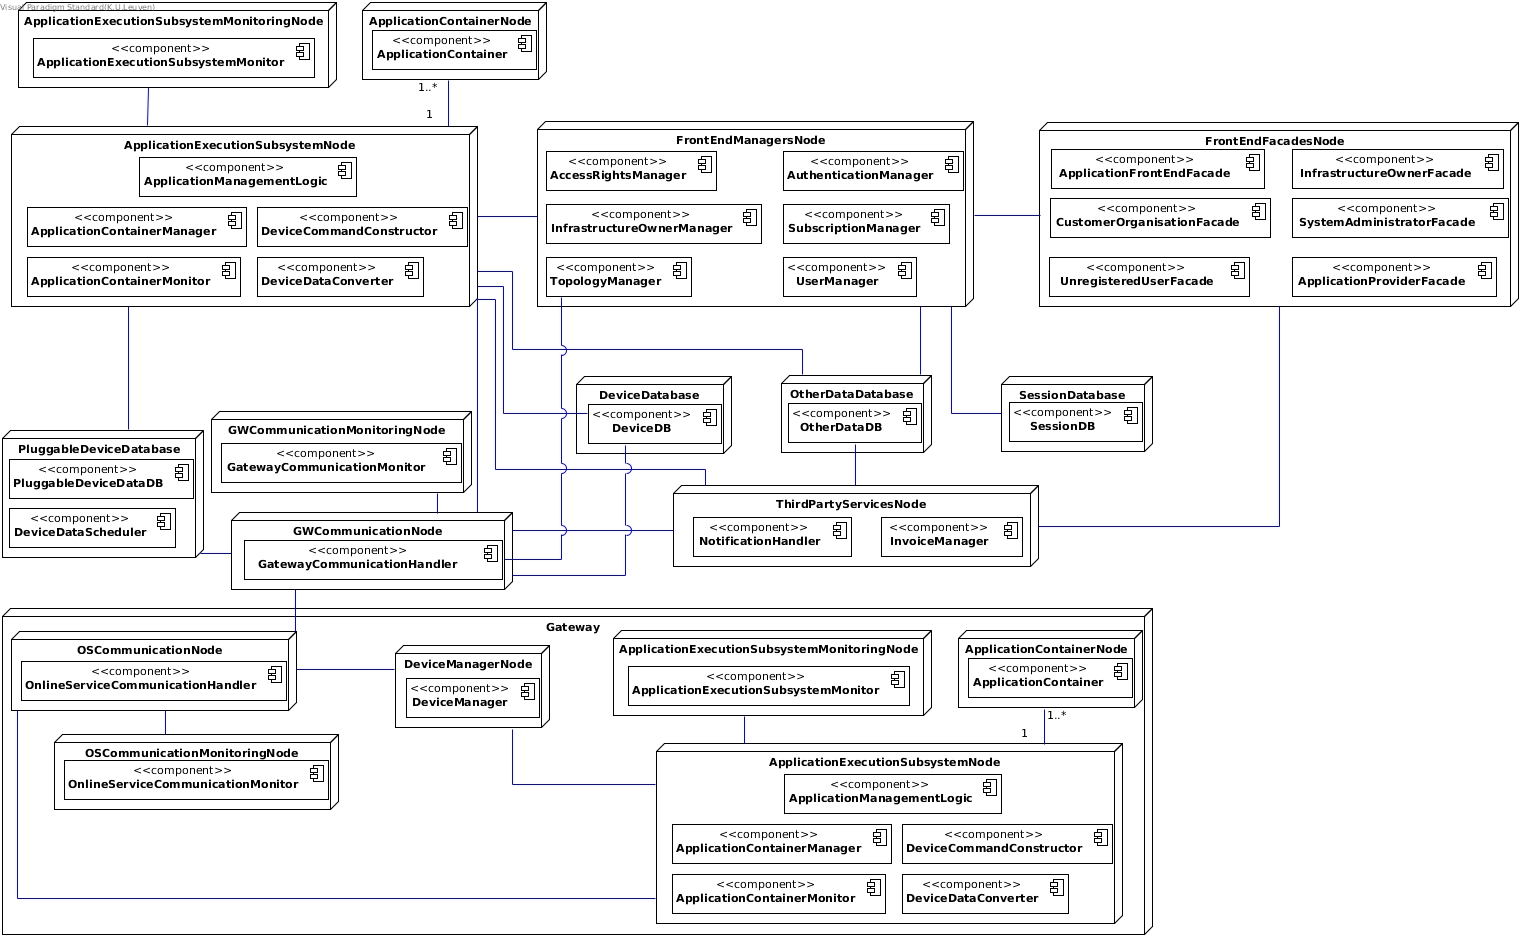
\includegraphics[width=\textwidth]{images/deployment-primary}
        	\caption{Primary diagram for the deployment view.}\label{fig:depl_primary}
        \end{figure}

    \vfill
\end{landscape}

    \clearpage

\chapter{Scenarios}\label{ch:scenarios}
    \minilof
    % \chapter{Scenarios}\label{ch:scenarios}

% Delete the command below to remove the hints and instructions
\showscenariosnotes{}

\todoinline{
	Illustrate how your architecture fulfills the most important data flows. As a rule of thumb, focus on the scenario of the assignment. Describe the scenario in terms of architectural components using UML Sequence diagrams and further explain the most important interactions in text. Illustrating the scenarios serves as a quick validation of the completeness of
	your architecture. If you notice at this point that for some reason, certain functionality or qualities are not addressed sufficiently in your architecture, it suffices to
	document this, together with a rationale of why this is the case according to you. You do not have to further refine you architecture at this point.}


\begin{figure}[!htp]
	\centering
	%\includegraphics[width=\textwidth]{}
	\missingfigure[figwidth=0.8\textwidth]{Sequence diagram scenario 1}
	\caption[Scenario 1]{The system behavior for the first scenario.}\label{fig:seq_scenario1}
\end{figure}


\chapter{Element Catalog and Datatypes}\label{ch:elements-datatypes}
    % \chapter{Element Catalog and Datatypes}\label{ch:elements-datatypes}

% Delete the command below to remove the hints and instructions
\showcatalognotes{}

\section{Element catalog}\label{app:catalog}
    \todoinline{
    List all components and describe their responsibilities and provided
    interfaces.
    Per interface, list all methods using a Java-like syntax and describe their
    effect and exceptions if any.
    List all elements and interfaces alphabetically for ease of navigation.
    }

    \componentItem{ComponentZ}{
    	\begin{itemize}[noitemsep,nolistsep]
    		\item \textbf{Responsibility:} Responsibilities of the component.
    		\item \textbf{Super-component:} The direct super-component, if any.
    		\item \textbf{Sub-components:} the direct sub-components, if any.
    	\end{itemize}
    	\subsubsection*{Provided interfaces}
    	\begin{itemize}[noitemsep,nolistsep]
    		\item InterfaceA
    		\begin{itemize}
    			\item \texttt{returntType1 operation1(ParamType param) throws SomeException}
    			\begin{itemize}
    				\item Effect: Describe the effect of the operation
    			\end{itemize}
    			%
    			\item \texttt{void operation2(ParamType2 param)}
    			\begin{itemize}
    				\item Effect: Describe the effect of the operation
    				\item Exceptions: None
    			\end{itemize}
    		\end{itemize}
    		%
    		\item InterfaceB
    		\begin{itemize}
    			\item \texttt{returntType2 operation3()}
    			\begin{itemize}
    				\item Effect: Describe the effect of the operation
    			\end{itemize}
    		\end{itemize}
    	\end{itemize}
    	}

    \componentItem{ComponentA}{
    	\begin{itemize}[noitemsep,nolistsep]
    		\item \textbf{Responsibility:} Responsibilities of the component.
    		\item \textbf{Super-component:} The direct super-component, if any.
    		\item \textbf{Sub-components:} the direct sub-components, if any.
    	\end{itemize}
    	\subsubsection*{Provided interfaces}
    	\begin{itemize}[noitemsep,nolistsep]
    		\item InterfaceC
    		\begin{itemize}
    			\item \texttt{returntType1 operation1(ParamType param) throws SomeException}
    			\begin{itemize}
    				\item Effect: Describe the effect of the operation
    			\end{itemize}
    			%
    			\item \texttt{void operation2(ParamType2 param)}
    			\begin{itemize}
    				\item Effect: Describe the effect of the operation
    			\end{itemize}
    		\end{itemize}
    		%
    		\item InterfaceD
    		\begin{itemize}[noitemsep,nolistsep]
    			\item \texttt{returntType2 operation3()}
    			\begin{itemize}
    				\item Effect: Describe the effect of the operation
    			\end{itemize}
    		\end{itemize}
    	\end{itemize}
    }

    % This will alphabetically print the list of components.
    \printComponents


\section{Common interfaces}
    \todoinline{If you have any common interfaces used by multiple components you may define them here and refer to them.}

\section{Defined Exceptions}
    \todoinline{Instead of describing the exceptions with each operation, you may define common exceptions here and refer to them from the operation definition.}

\section{Defined data types}\label{app:datatypes}
    \todoinline{
    List and describe all data types defined in your interface specifications. List
    them alphabetically for ease of navigation.
    }

    \begin{itemize}
    	\item \texttt{Paramtype1}: Description of data type.
    	\item \texttt{Paramtype2}: Description of data type.
    	\item \texttt{returnType1}: Description of data type.
    \end{itemize}


\end{document}
